\documentclass[a4paper 12pt]{article}

\usepackage{fullpage} % Package to use full page
\usepackage{parskip} % Package to tweak paragraph skipping
\usepackage{tikz} % Package for drawing
\usepackage{amsmath}
\usepackage{hyperref}

%\usepackage{sketch}
\begin{document}

\title{REPORT \#2 \\
   Numerical Methods in Solid and Fluid Mechanics}
\author{Claudio Pierard \\ Ekene Alexander Abanobi}
\date{21/12/2018}

\maketitle

%%%%%%%%%%%%%%%%%%%%%%%%%%%%%
%%%%%%%%%%%%%%%%%%%%%%%%%%%%%
\section{Aims and Objectives}
The objective of this practical work was modelling a distribution chain of a car under tension, and perform a static structural analysis in 3D. In particular, we wanted to calculate the maximum tensile stress applied to the chain considering a safety factor.

%%%%%%%%%%%%%%%%%%%%%%%%%%%%%
%%%%%%%%%%%%%%%%%%%%%%%%%%%%%
\section{Synthesis of the Study}

The chain distribution of a car consists of four types of pieces assembled together. In figure~\ref{fig:chain_scan} is possible to see the way in the four pieces are assembled to form the chain. In the figure, we can highlight that there are two types of links, an external one and an internal one.

%%%%%%%%%%%%%%%%% chain_scan %%%%%%%%%%%%%%%%%%%%%%%%%
\begin{figure}[!ht]
    \centering
    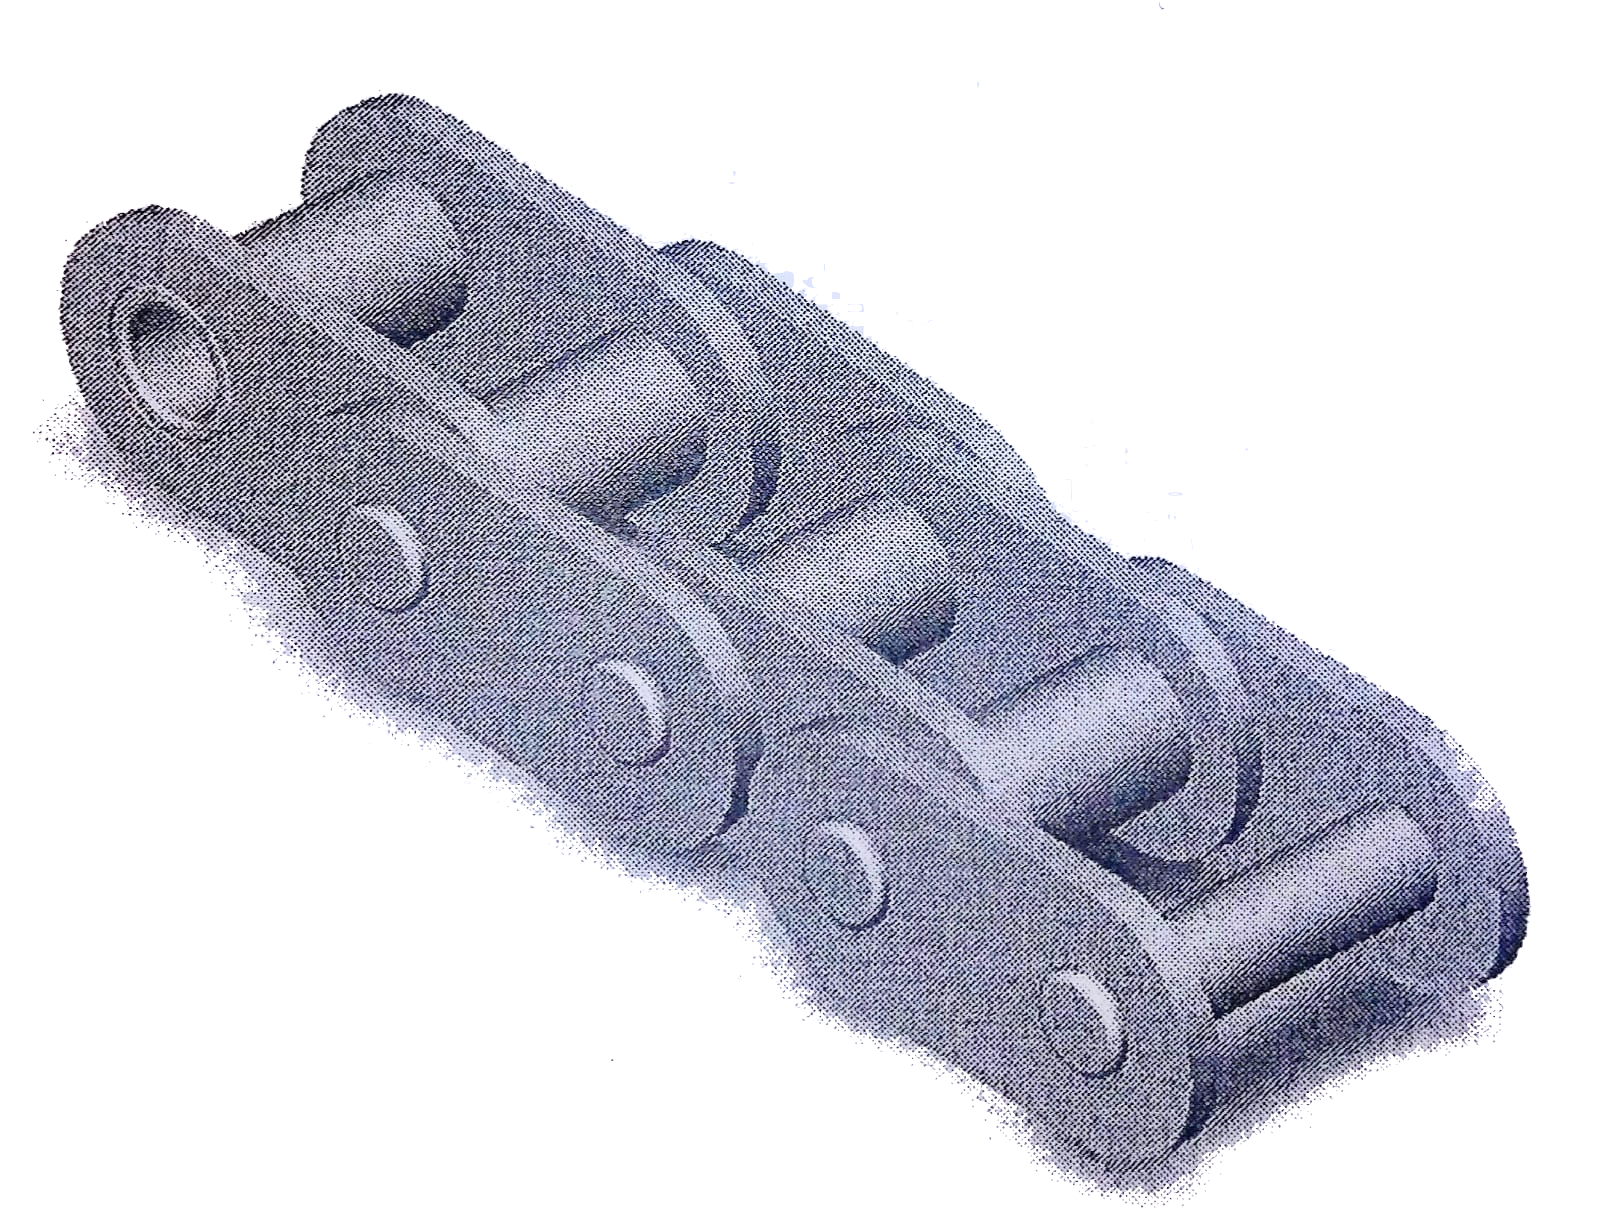
\includegraphics[width = 4cm]{images/chain_scan.png}
    \caption{Section of the distribution chain. It is possible to see the assembling of the pieces to form the chain.}
    \label{fig:chain_scan}
\end{figure}
%%%%%%%%%%%%%%%%%%%%%%%%%%%%%%%%%%%%%%%%%%%%%%%%%%%%%%%%%%%

The four pieces that make up the chain are shown in figure~\ref{chain_components}. From it, we distinguish two plates, one axis and one socket. In figure~\ref{fig:chain_scan} we can distinguish two types of plates in the chain. The plate A that is placed in the inner part of the chain, we call it inner plate, and the plate B placed in the outer part of the chain, we call it outer plate. Also, in figure~\ref{chain_components} we can see the axis, which correspond to the piece C, and the socket, which corresponds to the piece D.

The materials of the components of the chain are steel of different kinds depending on the part. For the plate, the material is steel XC55 with an elastic limit of 550~MPa. For the axis, the stell is XC65 with an elastic limit of 610~MPa. For the socket, the steel is 18CD4 with an elastic limit of 750~MPa.

%%%%%%% Chain links Sketch %%%%%%%%%
\begin{figure}[!ht]
\begin{center}
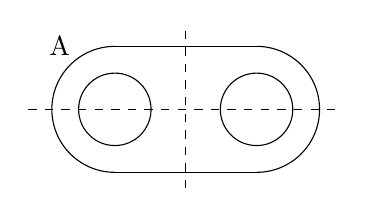
\begin{tikzpicture}[scale=0.2]
%\draw[red, thick, domain=0:2] plot(\x,0 * \x);
\draw [thin, -] (-4.5,4) -- (4.5,4);
\draw [thin, -] (-4.5,-4) -- (4.5,-4);
\draw (4.5,4) arc (90:-90:4);
\draw (-4.5,4) arc (90:270:4) (-8,4) node {A};
\draw(4.5,0) circle (2.3);
\draw(-4.5,0) circle (2.3);
\draw[thin,dashed] (-10,0) -- (10,0);
\draw[thin,dashed] (0,5) -- (0,-5);
\end{tikzpicture}
\qquad
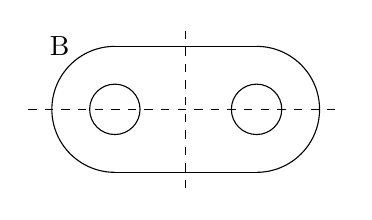
\begin{tikzpicture}[scale=0.2]
%\draw[red, thick, domain=0:2] plot(\x,0 * \x);
\draw [thin, -] (-4.5,4) -- (4.5,4) node [align=left, below]{};
\draw [thin, -] (-4.5,-4) -- (4.5,-4) node [align=left, below]{};
\draw (4.5,4) arc (90:-90:4);
\draw (-4.5,4) arc (90:270:4) (-8,4) node {B};
\draw(4.5,0) circle (1.6);
\draw(-4.5,0) circle (1.6);
\draw[thin,dashed] (-10,0) -- (10,0);
\draw[thin,dashed] (0,5) -- (0,-5);
\end{tikzpicture}
\qquad
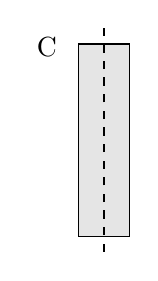
\begin{tikzpicture}[scale=0.2]
\filldraw[fill=gray!20](0,0) rectangle (3.25, 12.2);
\draw[thin,dashed] (1.625,-1) -- (1.625,13.2) (-2,12) node {C};
\end{tikzpicture}
\qquad
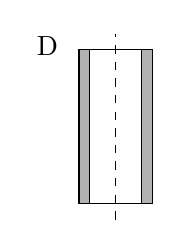
\begin{tikzpicture}[scale=0.2]
\filldraw[fill=gray!60] (0,0) rectangle (4.65,9.8) (-2,10) node {D};
\filldraw[fill=white!40] (0.675,0) rectangle (3.975,9.8);
\draw[thin,dashed] (2.325,-1) -- (2.325,10.8);
\end{tikzpicture}
\end{center}
\caption{The Four pieces that make up the chain. A is the inner plate, B is the outer plate, C is the axis and D is the socket.}
\label{chain_components}
\end{figure}
%%%%%%%%%%%%%%%%%%%%%%%%%%%%%%%%%%%%

The chain is under tension by means of pinions, which drive it at low speed to consider a static structural analysis. In other words, we assume that the chain is static and a force is applied in the direction along the chain moves.

%%%%%%%%%%%%%%%%%%%%%%%%%%%%%
%%%%%%%%%%%%%%%%%%%%%%%%%%%%%
\section{Methodology}

For modelling the chain we used ANSYS, which is software for 3D designing and performing simulations in a wide variety of problems. In this case, we used it to perform a static structural analysis of the chain. Maybe to do this we could have drawn all the components of the whole chain to model the entire chain, so the study would have been more realistic. The problem in doing this is that it would have taken us too much time, and the computational time for simulating the dynamics would have been very large. Instead of doing this, we reduced the problem to the fundamental pieces, taking into account that the same parts of the chain repeat them self many times. Also, we used the symmetries present in the chain to reduce the problem in the fundamental parts, and from them, infer the behaviour of the whole chain.

The first symmetry that we used to reduce the problem was the one that separates both sides of the chain in the direction were the chain moves. There are two sides that are symmetric that make up the chain, a pair of inner plates connected by the sockets and a pair of outer plates connected by the axis, and so on all along the chain. In this was, we are able to model just one side of the chain.

Figure~\ref{chain_union} is a sketch of the simplest connection of the chain that includes all the different parts. In this figure, we can see at the left the inner plate with the socket. Overlapped to the inner plate we see the outer plate with the axis. Also, we can see three dashed lines that cut through the chain. These lines are the axis of symmetry of the chain span and separate the chain span in 6 regions (labels 1 to 6). Parallel to the x-axis, we can see that there is an axis of symmetry in which the top part and the bottom part are similar. In other words, the regions 1, 2 and 3 are equivalent to the regions 4, 5, 6.

%%%%%%% Chain links Sketch %%%%%%%%%
\begin{figure}[!htbp]
\begin{center}
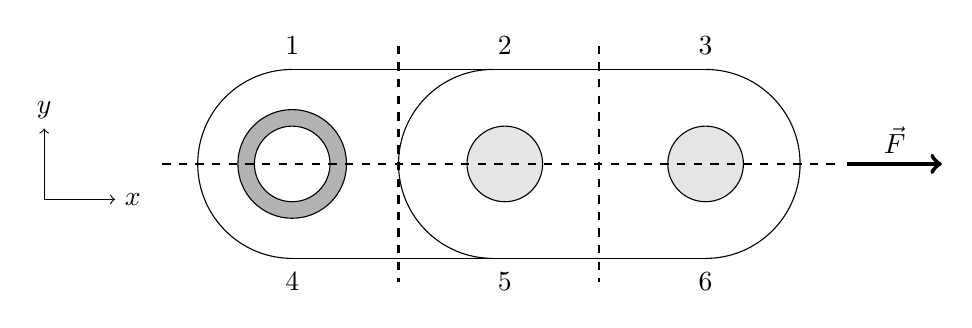
\begin{tikzpicture}[scale=0.3]
\draw [thin, -] (-4.5,4) -- (4.5,4);
\draw [thin, -] (-4.5,-4) -- (4.5,-4);
%\draw (4.5,4) arc (90:-90:4);
\draw (-4.5,4) arc (90:270:4);
\filldraw[fill=gray!20](4.5,0) circle (1.6) (-4.5,5) node {1};
\filldraw[fill=gray!60](-4.5,0) circle (2.3)(-4.5,-5) node {4};
\filldraw[fill=white!20](-4.5,0) circle (1.6)(4.5,5) node {2};
\draw [thin, -] (4,4) -- (13,4)(4.5,-5) node {5};
\draw [thin, -] (4,-4) -- (13,-4)(13,5) node {3};
\draw (13,4) arc (90:-90:4)(13,-5) node {6};
\draw (4,4) arc (90:270:4);
\filldraw[fill=gray!20](13,0) circle (1.6);
\draw[thick,dashed] (-10,0) -- (18.5,0);
\draw[thick,dashed] (0,5) -- (0,-5);
\draw[thick,dashed] (8.5,5) -- (8.5,-5) (21,1) node {$\Vec{F}$};
\draw[ultra thick, ->] (19,0) -- (23, 0);
\draw[->] (-15,-1.5) -- (-12,-1.5) node[right] {$x$};
\draw[->] (-15,-1.5) -- (-15,1.5) node[above] {$y$};
\end{tikzpicture}
\end{center}
\caption{Schematic of the section of consideration of the chain. The dashed lines are the axis of symmetry. From it, we can see that the section of consideration is divided into 6 sections (numbered in the top and bottom of sections). A force $\vec{F}$ is applied in the $x$-direction. The schematic is in the $y$-$x$ plane, with the $z$-axis coming outside of the page.}
\label{chain_union}
\end{figure}
%%%%%%%%%%%%%%%%%%%%%%%%%%%%%%%%%%%%

In figure~\ref{chain_union} as well, we can see two axes of symmetry parallel to the y-axis, in which the regions 1, 2 and 3 are similar (considering that there is an outer plate on region 1 and 4). This means that for studying the whole chain we can only simulate the region 2, in which the four different parts of the chain are involved. This implies that in the simulation we must only consider a quarter of each plate, and a semi-section of the axis and the socket. Also, is important to highlight that the force is applied in the positive x-direction.

Once we simplified as much as possible the problem, we proceeded to do the do the analysis of the reduced parts of the chain. The chain links are connected with the socket and the axis. The outer plate is fixed to the axis, and the inner plate is fixed to the socket. The axis goes inside of the socket and these two pieces are movable, which gives the chain its freedom of movement in the y-direction. In the static analysis is complex to perform the study of the four parts, including the movables parts. For this reason we decided to treat each piece separately and link each piece using the boundary conditions that correspond to each one of the pieces. Thereby, we explain separately the condition under which we made the analysis for each piece.

\subsection{Inner plate}

As already explained before, we took only a quarter of the plate because of the symmetries. We considered one of the superior quarters. To perform the analysis we draw this piece in ANSYS workbench, and introduced the material properties like the elastic limit. 

Following this, we established the boundary conditions for the surfaces of the plate as follows:

\begin{itemize}
  \item \textit{Bottom surface}: the surface is fix in the y-direction but is free to move in the x and z directions.
  \item \textit{Arc (surface inside the semicircle)}: In this surface we applied the force in the positive x-direction.
  \item \textit{Lateral surfaces}: the lateral surfaces are free to move in the three directions.
  \item \textit{Side surface (symmetry with respect of the y-axis)}: this surface is set to move free in the y and z directions, but it cannot move in the x direction. This boundary condition opposes the force and with this we avoid the rigid body movement of the plate.
  
\end{itemize}

Finally we performed the simulation, obtaining the stress and the displacement.

\subsection{Outter plate}

As well as for the inner plate we set up the material property and draw the geometry of only the superior quarter of the plate. Following this, we established the boundary conditions and performed the numerical simulation, obtaining the stress and the deformation. 

The boundary conditions used for this plate were the same as for the inner plate. 

\begin{itemize}
  \item \textit{Bottom surface}: the surface is fix in the y-direction but is free to move in the x and z directions.
  \item \textit{Arc (surface inside the semicircle)}: In this surface we applied the force in the positive x-direction.
  \item \textit{Lateral surfaces}: the lateral surfaces are free to move in the three directions.
  \item \textit{Side surface (symmetry with respect of the y-axis)}: this surface is set to move free in the y and z directions, but it cannot move in the x direction (avoiding rigid body movement).
  
\end{itemize}

\subsection{Axis}

For this part we divided the axis in two parts: the section that is in contact with the outer plate and the rest of the axis (until the middle). The outer part is what really interests us because the outer plate creates a shear force in the axis. The interior section of the section act as an anchor to this shear force. Also, the interior section of the axis will not deform because is enclosed by two inner plates that exert the same force in the same direction. So the main deformation and stress will be in the outer section of the piece. Hence we considered only the outer part of the axis.

We divided the outer part of the axis in two parts (semi-cylinders), because there is only symmetry with respect to the x-direction, considering the symmetries in section 2 of figure~\ref{chain_union}. The boundary conditions for this piece of the axis are:

\begin{itemize}
\item \textit{Bottom surface}: Fixed in the y component. This is so because the force is applied along the x-direction and hence x-direction cannot be constrained as it will cause an overconstrained system. It was also not be constrained in the z-direction because that is the axis the deformation will tend to.

\item \textit{Top surface (arc)}: In this surface the force is applied in the x-direction.

\item \textit{Inner Lateral surface}: This is fixed in the x and z directions
This surface is fixed in the x-direction even though the force is applied in the x-direction, because we do not want rigid body motion. It is also fixed in the z-direction because we are stating that the body under consideration is continuous in the z-direction i.e. taking into consideration that the axis has a length larger than the portion we are considering.

\item \textit{Outer Lateral Surface}: This is free to move in all directions. There are no constraints in this surface.

\end{itemize}

\subsection{Socket}

The socket is only in contact with the inner plate, so we analysed only this section, equivalent to the thickness of the inner plate. The boundary conditions for this part are:

\begin{itemize}
    \item \textit{Bottom surfaces}: As well as in the last three parts, this surfaces (there are two in the bottom) are fixed in the x-direction and free to move in the remaining two. 
    \item \textit{Inner lateral surface}: this surface is where we cut the socket just to consider the section in contact with the inner plate. Because of this, the surface is fixed in the x and z direction, but is free to move in the y direction. This is the anchor for or simulation. 
    \item \textit{Outer lateral surface}: This surface is free to move in all the three principal directions, assuming that the outer plate is not in contact with this socket.
    \item \textit{Top arc surface}: This surface is enclosed by the inner plate, so it cannot move in the y and x directions, only in the z direction. This constraints are the anchor point for the piece to avoid free body motion.
    \item \textit{Inner arc surface}: The force is applied in the x-direction in this surface.
\end{itemize}

%%%%%%%%%%%%%%%%%%%%%%%%%%%%%
%%%%%%%%%%%%%%%%%%%%%%%%%%%%%

\section{Link hypothesis}

In the four simulations made for the different parts of the chain, we determined the maximum stress each piece can hold before reaching the elastic limit. For this, we computed the theoretical max stress using the elastic limit for each material, and we divided it by the safety factor 1.3 (provided). Having the theoretical maximum stress, we performed the simulation changing the force applied to each one of the pieces of the chain, and we where able to find the force necessary to reach the maximum stress. The results are displayed in the results section, in table~\ref{table:results}. 

%%% READ the article that I sent you of the stress in the bycicke chain, we are going to use the same hypothesis to link both simulations.

To link the results of the simulation done for each one of the chain parts, we had to reconstruct the pieces that we cut with the help of the geometry of the chain. The way to link all the hypothesis is computing the total force applied to the whole chain. For doing this, we selected the smallest force of the pieces necessary to reach the maximum stress. This is the force that will be applied to all the reduced parts. Using this value of the force, we know that the section that we analysed was composed of four plates (two inner and two outer plates), one axis and one socket. The total force applied to the chain will be four times the corresponding force to reach the maximum stress on the weakest part of the chain. This meas that:

\begin{equation}
    \vec{F}_{Total} = 4 \vec{F}_{M.S.}.
\end{equation}

This is because the the force is evenly distributed between the four plates that compose each chain link. The total force computed is shown in the results section. 

%%%%%%%%%%%%%%%%%%%%%%%%%%%%%
%%%%%%%%%%%%%%%%%%%%%%%%%%%%%
\section{Results and Discussion}

In this section we show the results obtained in the numerical simulations obtained for the the four pieces. In special we show the deformation and the equivalent Von Mises stress.

\subsection{Outer Plate}
We can see from fig. \ref{fig:outer_deformation} that the displacement is tending towards the positive x-axis. This is a clear indication of the fact that we applied the force along the positive x-axis. Maximum displacement is experienced at the end as the displacement can be modelled as a linear function which increases with increasing length. A maximum displacement of about 8mm was seen for the applied force of 378N.   



%%%%%%%%%%%%%%%%%%% Outer plate %%%%%%%%%%%%%%%%%%%%%%%%%
\begin{figure}[!ht]
    \centering
    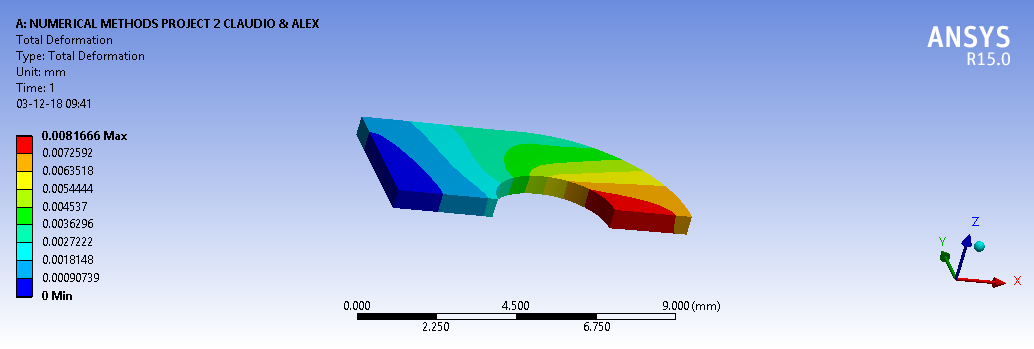
\includegraphics[width=1\textwidth]{images/OUTER_CHAIN_DEFORMATION.png}
    \caption{Deformation in the outer plate. Units are in millimetres.}
    \label{fig:outer_deformation}
\end{figure}

Also from fig. 5 below a maximum equivalent Von-Mises stress of 422.5MPa was obtained. An interesting point to note is the region of action of that maximum stress. 

\begin{figure}[!ht]
    \centering
    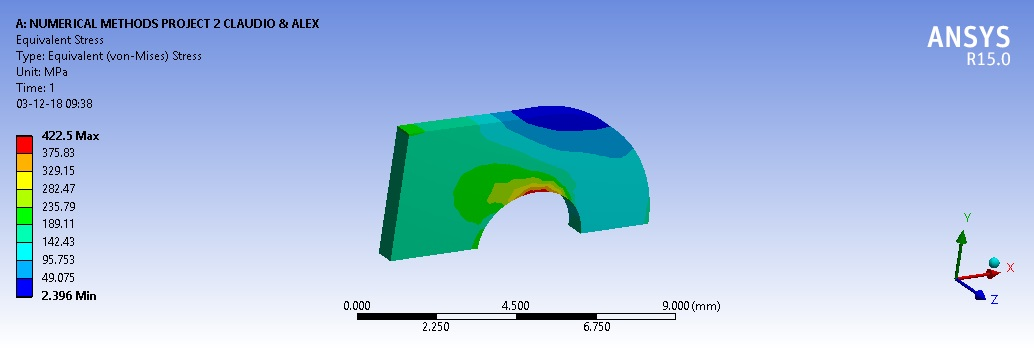
\includegraphics[width=1\textwidth]{images/CHAIN_SMALL_STRESS_TEST_FINAL.jpg}
    \caption{Equivalent stress in the outer plate. Units are in mega pascals (MPa).}
    \label{fig:outer_stress}
\end{figure}
%%%%%%%%%%%%%%%%%%%%%%%%%%%%%%%%%%%%%%%%%%%%%%%%%%%%%%%%%%%

\newpage
\subsection{Inner Plate}

%%%%%%%%%%%%%%%%%%%%%%% Inner plate %%%%%%%%%%%%%%%%%%%%%%%%
\begin{figure}[!ht]
    \centering
    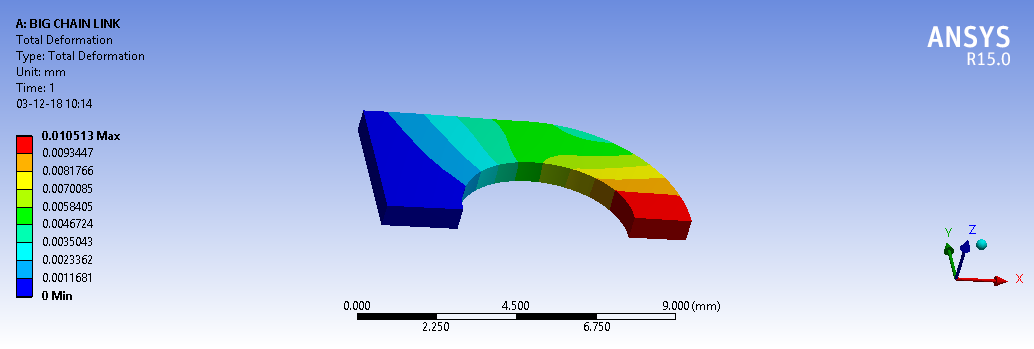
\includegraphics[width=1\textwidth]{images/INNER_CHAIN_DEFORMATION.png}
    \caption{Deformation in the inner plate. Units are in millimetres.}
    \label{fig:inner_deformation}
\end{figure}

\begin{figure}[!ht]
    \centering
    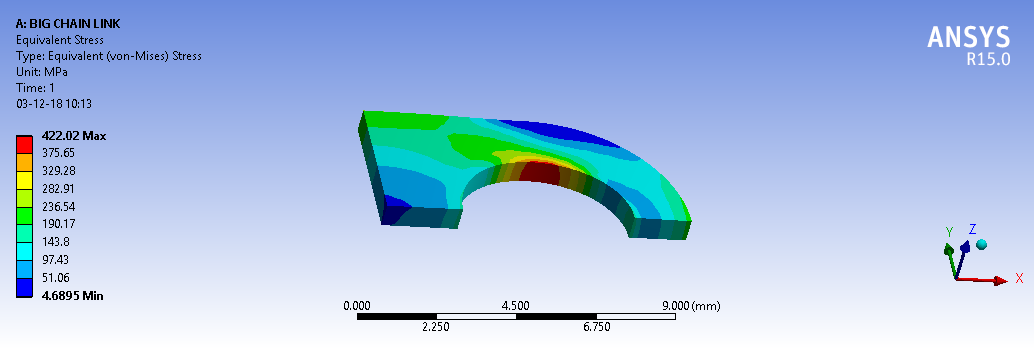
\includegraphics[width=1\textwidth]{images/INNER_CHAIN_STRESS.png}
    \caption{Equivalent stress in the inner plate. Units are in mega pascals (MPa).}
    \label{fig:inner_stress}
\end{figure}
%%%%%%%%%%%%%%%%%%%%%%%%%%%%%%%%%%%%%%%%%%%%%%%%%%%%%%%%%%%

\newpage
\subsection{Axis}

%%%%%%%%%%%%%%%%%%%%%%% Axis %%%%%%%%%%%%%%%%%%%%%%%%
\begin{figure}[!ht]
    \centering
    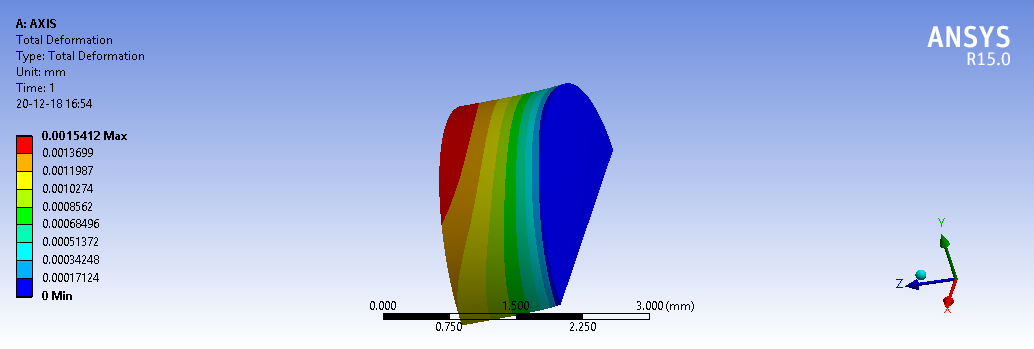
\includegraphics[width=1\textwidth]{images/AXIS_DISPLACEMENT.png}
    \caption{Deformation in the outer section of the axis. Units are in millimetres.}
    \label{fig:axis_deformation}
\end{figure}

\begin{figure}[!ht]
    \centering
    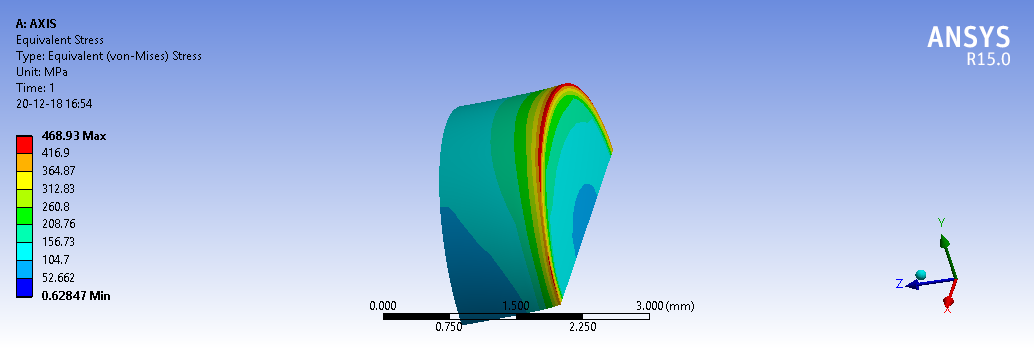
\includegraphics[width=1\textwidth]{images/AXIS_STRESS.png}
    \caption{Equivalent stress in the section of the axis. Units are in mega pascals (MPa).}
    \label{fig:axis_stress}
\end{figure}
%%%%%%%%%%%%%%%%%%%%%%%%%%%%%%%%%%%%%%%%%%%%%%%%%%%%%%%%%%%
\newpage
\subsection{Socket}

%%%%%%%%%%%%%%%%%%%%%%% Socket %%%%%%%%%%%%%%%%%%%%%%%%
\begin{figure}[!ht]
    \centering
    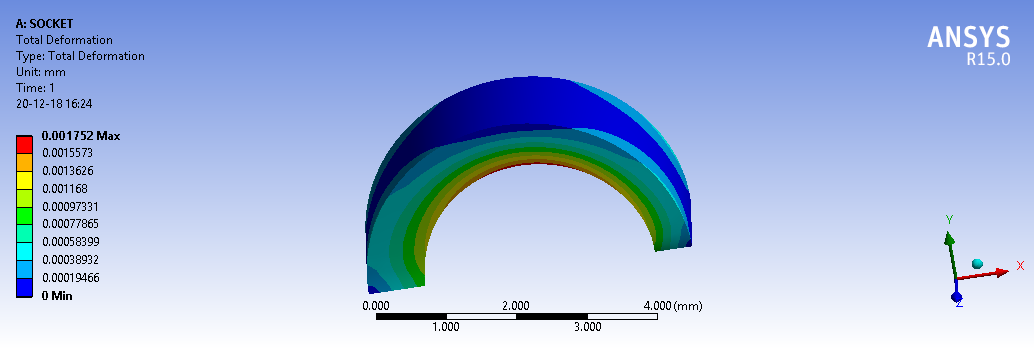
\includegraphics[width=1\textwidth]{images/SOCKET_DEFORMATION.png}
    \caption{Deformation in the socket. Units are in millimetres.}
    \label{fig:socket_deformation}
\end{figure}

\begin{figure}[!ht]
    \centering
    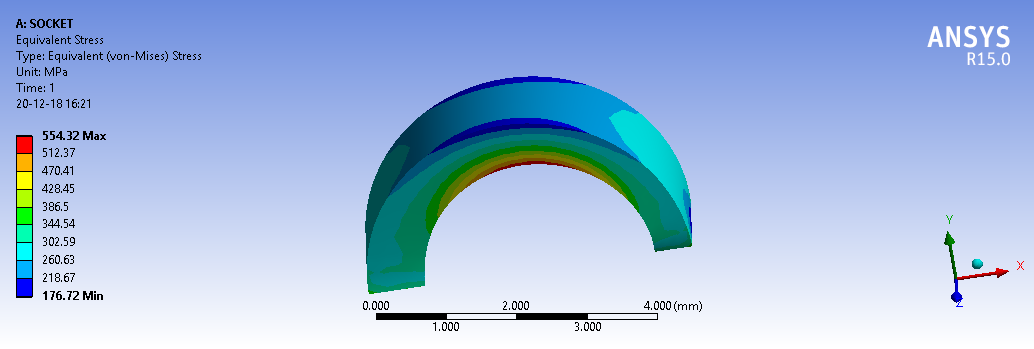
\includegraphics[width=1\textwidth]{images/SOCKET_STRESS.png}
    \caption{Equivalent stress in the socket. Units are in mega pascals (MPa).}
    \label{fig:socket_stress}
\end{figure}
%%%%%%%%%%%%%%%%%%%%%%%%%%%%%%%%%%%%%%%%%%%%%%%%%%%%%%%%%%%

\newpage
%%%%%%%%%%%%%%%%%%%% TABLE %%%%%%%%%%%%%%%%%%%%%%%%%%%%%%%%%%
\begin{table}
%\centering
\begin{center}
\begin{tabular}{|p{4cm}|c|c|c|c|}
\hline
  & \textbf{Outer Plate} & \textbf{Inner Plate} & \textbf{Axis} & \textbf{Socket} \\
\hline
Max. Force (Elastic Limit) [N] & 378 & 368 & 404.2 & 2500 \\
\hline
Theoretical Stress considering Elastic Limit [MPa] & 423 & 423 & 469 & 576 \\
\hline
Equivalent Von-Mises Stress [MPa] & 422.5 & 422.02 & 468.93 & 554 \\
\hline
\end{tabular}
\caption{Comprehensive table of results}
\label{table:results}
\end{center}
\end{table}

%%%%%%%%%%%%%%%%%%%% END OF TABLE %%%%%%%%%%%%%%%%%%%%%%%%%%%


\section{CONCLUSION}

%\bibliographystyle{plain} %We don't have references, I think...
%\bibliography{bibliography.bib}
\end{document}
